\documentclass[class=report, crop=false, a4paper, 12pt]{standalone}

%Packages import
\usepackage{../pkgs}


\begin{document}
\newpage
% A face recognition system works in either or both of two modalities: face verification (or authentication) or face identification (or recognition). The difference between them lies in the final stage of the workflow, identification involves a one-to-one pairing, while identification is a one-to-many match.

\section{Face Recognition}
Face Recognition (FR) is a thoroughly debated and extensively researched task in the Computer Vision community for more than two decades \autocite{ranjanDeepLearningUnderstanding2018}, popularized in the early 1990s with the introduction of the Eigenfaces \autocite{turkEigenfacesRecognition1991} or Fisherfaces \autocite{p.n.belhumeurEigenfacesVsFisherfaces1997} approaches. These methods projected faces in a low-dimensional subspace assuming certain distributions, but lacked the ability to handle uncontrolled facial changes that broke said assumptions, henceforth, bringing about face recognition approaches through local-features \autocite{chengjunliuGaborFeatureBased2002, ahonenFaceDescriptionLocal2006} that, even though, presented considerable results, weren't distinctive or compact. Beginning in 2010, methods based on learnable filters arose \autocite{z.caoFaceRecognitionLearningbased2010,leiLearningDiscriminantFace2014}, but unfortunately revealed limitations when nonlinear variations were at stake.

\par Earlier methods for FR worked appropriately when the data was handpicked or generated on a constrained environment, however, they didn't scale adequately in the real world were there are large fluctuations in, particularly, pose, age, illumination, background scenario, the presence of facial occlusion \autocite{ranjanDeepLearningUnderstanding2018} and many unimaginable more. These shortcomings can be dealt with by using Deep Learning, a framework of techniques that solves the nonlinear inseparable classes problem \red{ref.}, more specifically a structure called Convolutional Neural Network (CNN) \autocite{wangDeepFaceRecognition2021}. 

\par CNNs are an Artificial Neural Network (ANN) that exhibit a better performance on image or video-based tasks compared to other methods \autocite{lecunGradientBasedLearningApplied1998}. They were greatly hailed in 2012, after the AlexNet \autocite{krizhevskyImageNetClassificationDeep2012} victory, by a great margin, in the ImageNet Large Scale Visual Recognition Challenge (ILSVRC). Just two years later, DeepFace \autocite{taigmanDeepFaceClosingGap2014} revolutionized the benchmarks scores by achieving state-of-the-art results that approached human performance, reinforcing even further the importance of Deep Learning and shifting the research path to be taken \autocite{wangDeepFaceRecognition2021}.

\par Given what has been stated so far and the proven robustness, performance, and overall results in computer vision \red{ref. won competitions}, the methods discussed in this dissertation will therefore deal exclusively with Deep Learning approaches. For more information on other methods, please refer to \autocite{learned-millerLabeledFacesWild2016}.
% The exponential growth in the Artificial Intelligence domain, its corresponding subfields and technologies involved, spanned a plethora of terms that can be easily confused, mistook or mixed. For a better understanding of this dissertation, before discussing methods and implementations, it's important to analyze the fundamentals.


% \vspace{\baselineskip}
% \noindent\textbf{Computer Vision} is the science of trying to mimic with a computer what the humans do when looking at a scene, that is, extracting information from images through a series of computational techniques. \autocite{szeliskiComputerVisionAlgorithms2022}

% \vspace{\baselineskip}
% \noindent\textbf{Image querying}, is the process of finding information in a database of images that corresponds to the user query\footnote{Query, in computer science, is the request for information in a database.}, in this case, an image query\autocite{bartoliniImageQuerying2009}.  

% \vspace{\baselineskip}
% \noindent\textbf{Face verification}, also referred to as \textbf{face authentication}, is a one-to-one match, and it's the action of verifying if the query face matches the identity that's being claimed. These principles are used in biometric systems such as self-service immigration clearance using E-passport. \autocite{liHandbookFaceRecognition2011}

% \vspace{\baselineskip}
% \noindent\textbf{Face identification}, also called \textbf{face recognition}, is a one-to-many correlation process that compares a query face to a database of faces and associates it to the corresponding match (or matches). A typical use case is to identify someone in a watchlist or surveillance videos. \autocite{liHandbookFaceRecognition2011} 

\section{A Face Recognition System}
According to Ranjan \textit{et al.} \autocite{ranjanDeepLearningUnderstanding2018}, the goal of a FR system is to find, process and learn from a face, gathering as much information as possible, and as a result, it is one of the most widely implemented biometric system solutions, in light of its versatility when facing real world application \autocite{duElementsEndtoendDeep2022}, such as \red{military, public security and daily life}.

\par By and large, all end-to-end automatic face recognition systems follow a sequential and modular\footnote{Sequential because each stage relies on the output from the previous ones, and modular in the sense that each stage employs its own method and it can be modified to better adapt to specific tasks.} pipeline composed of three pillar stages \autocite{wangDeepFaceRecognition2021}: face detection, face alignment and face representation. First an image or video feed is used as an input then, as the name suggests, the face detection module is responsible for finding a face. Next, the face alignment phase applies transformations to the data, such as crop and/or rotation, in order to normalize the faces' pictures (or frames, in the case where a video is used) to standardized coordinates. Finally, the face representation stage, makes use of deep learning techniques to learn discriminative features that will allow the recognition.

\par All three stages have their individual importance and methods of implementation\footnote{For a deeper and extensive study, please refer to: \autocite{zafeiriouSurveyFaceDetection2015} in the case of classic face detection approaches and \autocite{minaeeGoingDeeperFace2021} for deep learning based methods; \autocite{wangFacialFeaturePoint2018} addresses traditional face alignment methods and is complemented with \autocite{duElementsEndtoendDeep2022} for more up-to-date techniques; and \autocite{learned-millerLabeledFacesWild2016} tackles classic ones \red{add if needed: while X supplements the deep learning methods}}. Face detection is achievable through classical approaches \autocite{violaRapidObjectDetection2001, brubakerDesignCascadesBoosted2008} or deep methods, among them is \autocite{dengRetinaFaceSingleShotMultiLevel2020} and the widely applied \autocite{zhangJointFaceDetection2016}. Face alignment, once again, can be accomplished through traditional measures \autocite{cootesViewbasedActiveAppearance2002, martinezLocalEvidenceAggregation2013} or more modern ones, namely \autocite{huangPropagationNetPropagatePoints2020} or the aforementioned \autocite{zhangJointFaceDetection2016} who concurrently performs detection and alignment. To conclude, the face representation module is no exception, and can also be divided in two groups, regarding the methodology used. Some conventional systems were already mentioned, such as \autocite{p.n.belhumeurEigenfacesVsFisherfaces1997,turkEigenfacesRecognition1991}, and the deep learning ones are the objective of discussion of this dissertation and will be reviewed along the following sections.


\section{Face Representation Pipeline}
\subsection{Convolutional Neural Networks} %Review this article \autocite{kangDeepSimilarityMetric2019}
There are several types of Neural Networks architectures, but Convolutional Neural Networks (CNNs or Convnets) are probably the most widely implemented model overall \autocite{yamashitaConvolutionalNeuralNetworks2018, liSurveyConvolutionalNeural2022} with successful applications in the domains of Computer Vision \autocite{krizhevskyImageNetClassificationDeep2012,taigmanDeepFaceClosingGap2014,tompsonEfficientObjectLocalization2015, zhangImprovedBreastCancer2021} or Natural Language Processing\autocite{abdel-hamidConvolutionalNeuralNetworks2014, wangGenCNNConvolutionalArchitecture2015, xiangConvolutionalNeuralNetworkbased2020}. In the CNN category itself there are different variants, but they all abide the fundamental structure of a feedforward hierarchical multi-layer network (Figure 1). Feedforward because the information only flows in a singular direction without cycling \autocite{zellSimulationNeuronalerNetze1994}, hierarchical because the higher complexity internal representations are learned from lower ones \autocite{lecunDeepLearning2015, zhuBCNNBranchConvolutional2017} and multi-layer because it is composed of a series of stages, blocks or layers: the raw data is fed to an input layer, forwarded to a sequence of intercalating convolutional and pooling layers, transmitted to a stage of one or more fully-connected layers \autocite{lecunDeepLearning2015, yamashitaConvolutionalNeuralNetworks2018, guRecentAdvancesConvolutional2018, alzubaidiReviewDeepLearning2021}. The convolutional layer is designed to extract feature representations by being composed of kernels (or filter banks \autocite{lecunDeepLearning2015}) that compute feature maps through element-wise product, to which is applied a nonlinear activation function \autocite{guRecentAdvancesConvolutional2018,yamashitaConvolutionalNeuralNetworks2018}. Next is the pooling layer, that's responsible for reducing the spatial size of the input data \autocite{guRecentAdvancesConvolutional2018} and joining identical features \autocite{lecunDeepLearning2015}. Finally, the fully connected layers, and their core function is to perform high logic and generate semantic information \autocite{guRecentAdvancesConvolutional2018}.

\begin{figure}[t!]
    \centering
    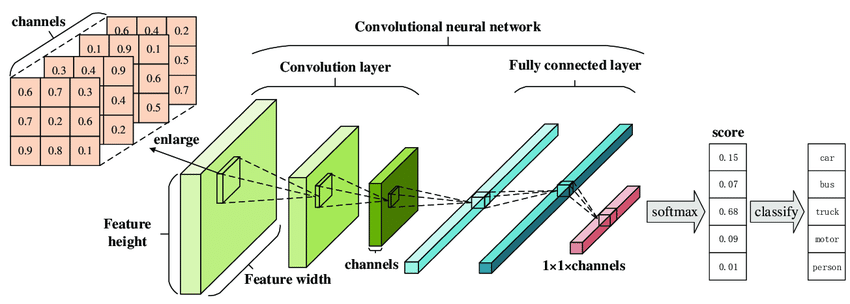
\includegraphics[scale=0.35]{Architecture-of-a-Convolutional-Neural-Network-CNN-The-traditional-CNN-structure-is.png}
    \caption{Architecture of a Convolutional Neural Network \autocite{kangDeepSimilarityMetric2019}}
\end{figure}

\par Using CNNs for Computer Vision tasks is not an arbitrary choice, but due to the fact that the network design can benefit from the intrinsic characteristics of the input data, consequently performing really well in image related applications \autocite{lecunDeepLearning2015,caoReviewNeuralNetworks2018}. In the first place, images have an array-like structure with numerous elements, namely, each pixel has an assigned value organized in a grid-like manner \autocite{yamashitaConvolutionalNeuralNetworks2018}. In the second place, there's an inherent correlation between local groups of values, which creates distinguishable motifs \autocite{lecunDeepLearning2015}. Finally, the local values of images are invariant to location, that is, a certain composition should have the same value independently of the spatial location in the picture \autocite{lecunDeepLearning2015}. Therefore, the following key, unique features potentiate the previously stated efficient performance \autocite{caoReviewNeuralNetworks2018}:
\begin{enumerate}
    \item Designed to process multidimensional arrays \autocite{lecunDeepLearning2015};
    \item Shared weights between the same features in different locations; %Invariance to shift, distortions and rotations
    \item Automatically identifies the relevant features without any human supervision, hence, small amounts of preprocessing \autocite{alzubaidiReviewDeepLearning2021,liSurveyConvolutionalNeural2022}; %Easier to train
    \item Local connections (or receptive fields/sparse connectivity) \autocite{alzubaidiReviewDeepLearning2021}; %Less complexity, easier to train; %Invariance to shift, distortions and rotations and less network complexity (easier to train)
    \item Pooling layers that reduces the spatial size of the input data. %Invariance to shift, distortions and rotations
\end{enumerate}
% Check this article for better description of key features \autocite{liSurveyConvolutionalNeural2022}

The ensemble of features 2, 4 and 5 enable an invariance of the network to small shifts, distortions and rotations \autocite{guRecentAdvancesConvolutional2018,lecunDeepLearning2015}, while 2, 3, 4 and 5 helps to reduce the complexity of the model, and as a result training it is easier\autocite{guRecentAdvancesConvolutional2018,liSurveyConvolutionalNeural2022}.
\end{document}